\section{Experiments}
\label{sec:exp}
We apply our research method experimentally on a large spatial-temporal dataset collected from IEEE dataport. By compare the result with real events in Coronanet which records government responses to coronavirus, we evaluate the plausibility of the method. The result shows several points of interest in a specific time period and the details within each topic.
\subsection{Dataset Description and Experiment Setup}
Dataset: \\
The dataset we used is CORONAVIRUS (COVID-19) GEO-TAGGED TWEETS DATASET form IEEE DataPort. Due to the tweets spreading policy. We can’t access the completed tweets directly. Thus. We use a transfer program named Twarc to batch fetch every tweet in the dataset. Twarc is a python package that is used to export tweets automatically. The main principle is that Twarc will make use of the registration information from twitter developer platform and get the permission from Twitter. Then Twitter can monitor the whole process of getting tweets. This way is completely legal and doesn’t violate the privacy protocols set by Twitter. But it also causes some issues. If the tweets account is banned or the permission has been changed, we can’t access the content anymore. Normally Twitter doesn’t send any warning message but changes the content of tweets to a prompt message. So some filtering process is necessary to ensure that the data set is not contaminated with irrelevant information.


Metrics:\\
We use silhouette factor to evaluate the performance of clustering. For storyline generation, we based on rationality of the time series and topic keywords. 


Topic mining:\\
To evaluate the quality of generated topics, we focus on both the content of the topic itself and the distribution of the topic. 


In the experiment, each topic consists of a series of related sentence vectors. We use high-frequency words in WordCloud to show the content of the topic. Besides, We also output one of the most representative sentences in each topic as supporting evidence. 


The distribution of clusters in the vector space is another indicator of the quality of the results. The projection of vectors in two-dimensional space can intuitively see the distribution of the cluster. In order to verify the temporal relevance of the topic we also use the time label of the topic vector as the third axis to generate a three-dimensional vector distribution map.


Comparison Models: \\
We propose a combination of lda and bert methods to produce high-quality sentence vectors. To verify the advantages of this approach, we output the clustering results using bert and LDA separately. We make a comprehensive assessment based on the quality of the topics and timelines generated by each method
\subsection{Results and Discussion}
\subsubsection{Derivation of topic}
\begin{figure}[h]
\centering
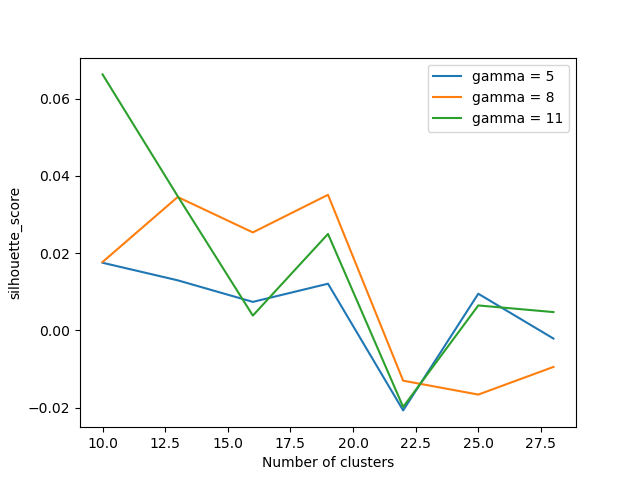
\includegraphics[width=0.5\textwidth]{imgs/2d_derivation.png}
\caption{2d derivation}
\label{fig:2d_derivation}
\end{figure}


\\In Fig~\ref{fig:2d_derivation}, we adjust the number of clusters and weight ratio of the vector structure to get the best silhouette score. The quality of the generated storyline will also be a reference. 
\subsubsection{Topic content}
\subsubsection{Evaluation of clustering}
\subsubsection{Storyline}
\subsubsection{Model comparision}

